\documentclass[english,twoside, openright, hidelinks, 11 pt, class=report,crop=false]{standalone}
\input{../../preamb}
\input{../bm}

\newcommand{\p}[1]{
\includegraphics[scale=0.3]{fig/#1}
}

\begin{document}
\chapter*{Kalkulator}
I dette kapitlet skal vi vise de grunnleggende metodene for å løse oppgaver med hjelp av en håndholdt kalkulator. Bildene viser bruk av en Casio FX 82 kalkulator, som innfrir Udirs nye krav til hjelpemidler på Del 2 av skriftlig eksamen i videregående skoler. I de fleste tilfeller vil fremgangsmåte og utseende være veldig lik også på andre kalkulatorer. Eksempler som viser bruk som er spesifikke for Casio FX 82 vil være markert.
\section*{Grunnleggende utregninger}
I figuren under vises utregning av utvalgte regnestykker Alle regnestykker avsluttes med knappen \p{enter}.

\begin{center}
	\begin{minipage}{0.48\linewidth}
		\begin{center}
			\begin{tabular}{l | l}
				$9\cdot3$ & \p{9}\p{times}\p{3} \\
				$5^2$ & \p{5}\p{x2}\\
				$\sqrt{25}$ & \p{sqrt}\p{2}\p{5} \\
				$\log_{10} 100$ & \p{log} \p{1}\p{0}\p{0} \\
				$7\pi$ & \p{7}\p{times}\p{pi}
			\end{tabular}
		\end{center}
	\end{minipage}
	\begin{minipage}{0.5\linewidth}
		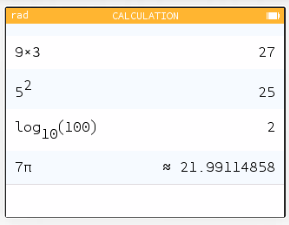
\includegraphics[scale=0.5]{fig/p1}
	\end{minipage}
\end{center}
\end{document}